% Stoa project scoping submission (IE7374 MLOps, Fall 2026).
% Source of truth for the scoping document; the PDF is a build artifact (untracked).
% Build: cd docs/scoping && latexmk -pdf -outdir=build project_scoping.tex && cp build/project_scoping.pdf .
\documentclass[11pt]{article}

\usepackage[letterpaper,margin=1in]{geometry}
\usepackage[T1]{fontenc}
\usepackage[utf8]{inputenc}
\usepackage[scaled=0.95]{helvet}
\renewcommand{\familydefault}{\sfdefault}
\usepackage{microtype}
\usepackage[table]{xcolor}
\usepackage{xltabular}
\usepackage{array}
\usepackage{enumitem}
\usepackage{titlesec}
\usepackage{fancyhdr}
\usepackage{caption}
\usepackage{float}
\usepackage{tikz}
\usetikzlibrary{positioning,calc,fit,backgrounds}
\usepackage[hidelinks]{hyperref}
\usepackage{xurl}

% ---------- Colours ----------
\definecolor{heading}{HTML}{1F3864}
\definecolor{subheading}{HTML}{2E5597}
\definecolor{headgray}{HTML}{E7E9EE}
\definecolor{rulegray}{HTML}{B4B9C3}
\definecolor{boxgray}{HTML}{F4F5F8}
\definecolor{boxline}{HTML}{9AA1AD}
\definecolor{bnfill}{HTML}{FDF0E6}
\definecolor{bnline}{HTML}{D9541E}
\definecolor{bntext}{HTML}{C2410C}
\definecolor{mlfill}{HTML}{E9F0FB}
\definecolor{mlline}{HTML}{3B73D1}
\definecolor{gatefill}{HTML}{EAF5EC}
\definecolor{gateline}{HTML}{3C8D4E}

% ---------- Headings ----------
\titleformat{\section}{\Large\bfseries\color{heading}}{\thesection.}{0.5em}{}
\titleformat{\subsection}{\large\bfseries\color{subheading}}{\thesubsection}{0.5em}{}
\titlespacing*{\section}{0pt}{14pt}{6pt}
\titlespacing*{\subsection}{0pt}{10pt}{4pt}

\setlength{\parindent}{0pt}
\setlength{\parskip}{6pt}
\setlist{itemsep=2pt,topsep=2pt,parsep=0pt}

\pagestyle{fancy}
\fancyhf{}
\renewcommand{\headrulewidth}{0pt}
\fancyfoot[C]{\small\color{gray}Page \thepage}

% ---------- Tables ----------
\arrayrulecolor{rulegray}
\renewcommand{\arraystretch}{1.25}
\newcolumntype{L}[1]{>{\raggedright\arraybackslash}p{#1}}
\newcolumntype{Y}{>{\raggedright\arraybackslash}X}
\newcommand{\hrow}{\rowcolor{headgray}}

\captionsetup{font={small,it},labelfont={small,it},justification=raggedright,singlelinecheck=false}


% ---------- Diagram styles ----------
\tikzset{
  stage/.style={draw=boxline, fill=boxgray, rounded corners=3pt, align=left,
                text width=#1, inner sep=4pt, font=\scriptsize, anchor=north west, minimum height=2.45cm,
                execute at begin node={\hyphenpenalty=10000\exhyphenpenalty=10000}},
  stage/.default=2.55cm,
  tall/.style={minimum height=3.0cm},
  bn/.style={draw=bnline, fill=bnfill},
  ml/.style={draw=mlline, fill=mlfill},
  gate/.style={draw=gateline, fill=gatefill},
  flow/.style={->, draw=boxline, >=stealth},
}
\newcommand{\bnlabel}[1]{\\[2pt]{\color{bntext}\bfseries\tiny #1}}
\newcommand{\mllabel}[1]{\\[2pt]{\color{mlline}\bfseries\tiny #1}}

\begin{document}

{\LARGE\bfseries\color{heading} Project Scoping Submission: Stoa}\par
\vspace{2pt}
\textit{Pedestrian flow prediction and scenario planning. IE7374 MLOps, Northeastern University, Fall 2026.}

\textbf{Team Members:}
\begin{itemize}
  \item Romit Basak
  \item Arshmehar Kaur
  \item Bimbasri Paduru
  \item Puneet Singh Puri
  \item Shubham Madhusudan Hadawle
\end{itemize}

% =====================================================================
\section{Introduction}

Stoa predicts where people walk, how many, and when, across the paths and streets of a site. Planners can then test a change before building it: close a path, add an entrance, or plan for a game day. They get back predicted hourly volumes for every path segment, with uncertainty bands.

Planners today have pedestrian counts at a handful of fixed sensors and almost nowhere else. Answering a what-if question usually means paying for manual counts and a consultant study, which takes weeks for a single scenario. Stoa learns the relationship between counts and the built environment where sensors exist. That includes network structure, slope, shade, destinations and their opening hours, visibility, weather, time and events. It then generalises to every unsensed segment and to edited versions of the network. How well it carries over to a new city is measured, not assumed (Section~\ref{sec:transfer}).

\textbf{Users:} city planners (primary), campus planners, event organisers (outdoor approach streets around venues only, never venue interiors), store owners choosing a site (``if I open here, how many people pass by, and when?''), and researchers (generic research mode with standard GIS exports).

\textbf{Case studies:}
\begin{itemize}
  \item \textbf{Melbourne (training and validation).} The City of Melbourne has run an automated pedestrian counting network since 2009. All accuracy claims rest here.
  \item \textbf{Melbourne transfer precincts (within-city transfer test).} Whole areas unlike the central business district are held out: the University of Melbourne edge, Carlton and North Melbourne.
  \item \textbf{New York City (cross-city transfer test).} The model is trained on Melbourne and tested on NYC DOT's open pedestrian counts. This is the only evidence for any claim beyond Melbourne.
  \item \textbf{Northeastern University Boston campus (demonstration).} No local ground truth, so the campus is a transfer demonstration, not an accuracy claim.
  \item \textbf{Event scenario (demonstration).} A stadium or campus event on the outdoor approach streets.
  \item \textbf{Marathons (stretch).} Melbourne Marathon as a validation case (course as closed edges with limited crossings); Boston Marathon as a demonstration (course as a barrier, spectator hotspots, leapfrogging spectators).
\end{itemize}

\textbf{ML components:} (1) a flow model predicting hourly volume per segment with prediction intervals, progressing from baselines to gradient-boosted trees (the learned model in scope; a spatio-temporal graph neural network is a stretch goal and must beat it to be adopted); (2) a path segmentation model that detects informal paths (desire lines) in aerial imagery and adds them to the network; (3) crowd simulation in two stages: route-sampling walkers driven by the flow model, then physics-style microsimulation for limited areas such as event egress zones and station approaches; (4) an LLM intake agent that turns natural-language requests and local knowledge into a structured scenario and narrates model outputs. The agents never produce numbers themselves. These sit inside a full MLOps loop: versioned data, tracked experiments, gated deployment, monitoring, and monthly retraining on new counts, with automated drift alerts and automated rollback safeguards.

% =====================================================================
\section{Dataset Information}

\subsection{Dataset Introduction}

The core dataset is the City of Melbourne Pedestrian Counting System. It provides hourly counts from automated sensors across the CBD, Southbank, Docklands, Carlton and North Melbourne, and it is the target variable for the flow model. Context layers explain why counts differ between places and times. They become model features, and they form the walking network the model predicts on. NYC DOT's counts are used only to test transfer to another city and never enter training.

\begin{xltabular}{\linewidth}{|L{3.6cm}|Y|L{3.4cm}|}
\hline\hrow
\textbf{Dataset} & \textbf{Purpose in the project} & \textbf{Provider} \\\hline
\endhead
Pedestrian counts (hourly) + sensor locations & Target variable: training, validation, monitoring & City of Melbourne (CoM) \\\hline
CoM Pedestrian Network & Walking graph: 71,060 typed links (footpaths, crossings with wait times, arcades, lanes) & CoM \\\hline
CoM footpath steepness, footpaths & Surveyed slope per footpath section; footpath width & CoM \\\hline
CoM building footprints 2023, CLUE census & Building heights for visibility; land use, jobs and floor space (trip generation) & CoM \\\hline
CoM trees and canopy, businesses, cafés, landmarks, transit, venues & Shade, destinations, transit access, event venues & CoM \\\hline
OpenStreetMap & Network for non-CoM sites (NEU, NYC), POIs, opening hours, crossings, entrances & OSM contributors \\\hline
GA 5\,m LiDAR DEM; Copernicus GLO-30; SRTM & Terrain for slope and the 3D viewshed & Geoscience Australia; ESA; NASA \\\hline
ESA WorldCover 2021 & Land cover (portable to sites without city layers) & ESA \\\hline
Hourly weather (ERA5 via Open-Meteo) & Temperature, rain, wind, radiation, daylight & Open-Meteo / ECMWF \\\hline
AFL games & Event days at the MCG and Marvel Stadium & Squiggle API \\\hline
Academic calendars & In-semester flag for segments near a university (University of Melbourne in training; NEU at serve time) & Universities (published calendars) \\\hline
NYC DOT Bi-Annual Pedestrian Counts & Cross-city transfer test only; never training & NYC DOT via NYC Open Data \\\hline
MassGIS 2025 orthos (15\,cm, leaf-off); NAIP 2023 (0.3\,m, leaf-on) & Path segmentation on the NEU campus. Leaf-off MassGIS is the primary input (paths under trees are visible); NAIP is the portable fallback & MassGIS / USDA \\\hline
USGS 3DEP 1\,m; City of Boston buildings & NEU terrain and building heights (2010 survey, in feet) & USGS / City of Boston \\\hline
Stanford Drone Dataset (planned) & Route-choice validation and an academic calibration demonstration; no model fine-tuned on it is shipped or distributed & Stanford \\\hline
Controlled pedestrian experiments (planned; e.g.\ the J\"ulich pedestrian dynamics data archive, to verify) & Microsimulation validation: speed--density measurements & Research archives \\\hline
\end{xltabular}

\subsection{Data Card}

\textbf{Primary dataset: Melbourne pedestrian counts}

\begin{xltabular}{\linewidth}{|L{3.6cm}|Y|}
\hline\hrow
\textbf{Property} & \textbf{Value} \\\hline
\endhead
Size & 6,186,603 sensor-hours: 4,562,230 (archive, 2009-05-01 $\rightarrow$ 2022-10-31) + 1,624,373 (live API, 2024-10-04 $\rightarrow$ present). $\sim$470\,MB uncompressed. \\\hline
Format & Archive: CSV in ZIP. Live: Parquet export from the Opendatasoft API. Sensor locations: GeoJSON. \\\hline
Granularity & One row per (sensor, local date, hour) \\\hline
Sensors & 103 with counts in the live window (100 outdoor + 3 retired); 82 in the archive; 67 overlap. 18 sensors in 2009 $\rightarrow$ 73 in 2022. \\\hline
Spatial extent & lon 144.929--144.986, lat $-37.826$ to $-37.789$ (inner City of Melbourne, $\sim$4\,$\times$\,5\,km) \\\hline
Gap & \textbf{No data Nov 2022 $\rightarrow$ Oct 2024 (23 months).} Neither source covers it. \\\hline
Distribution & Mean 394/h, median 160/h, max 6,632/h; right-skewed. Peaks 12:00--13:00 and 17:00; minimum $\sim$04:00. The median sensor's median hour is $\sim$210; only about a quarter of sensors sit below 100/h, so quiet paths are thin in the data. \\\hline
Quality & No negative values; total = direction 1 + direction 2 on every row; $\sim$90\% of sensor-hours present in the live window (outages are missing rows, not zeros); 11,730 duplicate keys in the archive (DST). \\\hline
Update cadence & Live API updated daily but kept as a \textbf{rolling $\sim$2-year window}: re-pulls are merged into the rows already held, never overwritten. Archive static. \\\hline
\end{xltabular}

\begin{xltabular}{\linewidth}{|L{3.6cm}|L{2.2cm}|Y|}
\hline\hrow
\textbf{Field (live export)} & \textbf{Type} & \textbf{Description} \\\hline
\endhead
location\_id & int & Sensor ID; equals Sensor\_ID in the archive \\\hline
sensing\_date & date & Local (Australia/Melbourne) date \\\hline
hourday & int 0--23 & Local hour \\\hline
direction\_1, direction\_2 & int & Directional counts (live window only) \\\hline
pedestriancount & int & Total count for the hour (target) \\\hline
sensor\_name & string & Short sensor code, e.g.\ Swa123\_T \\\hline
location & geo point & Sensor latitude/longitude \\\hline
\end{xltabular}

\textbf{Transfer-test dataset: NYC DOT Bi-Annual Pedestrian Counts} (checked 2026-10-04)

\begin{xltabular}{\linewidth}{|L{3.6cm}|Y|}
\hline\hrow
\textbf{Property} & \textbf{Value} \\\hline
\endhead
Locations & 114: 100 on-street (mostly retail corridors), 13 East River and Harlem River bridges, the Hudson River Greenway. All five boroughs. \\\hline
Sampling & Twice a year (May and September/October). One weekday (07:00--09:00 and 16:00--19:00) and the adjacent Saturday (12:00--14:00). Mid-block screenline, both sides of the street. \\\hline
Values & One total per location per period (AM, PM, Saturday midday), not hourly. A value of 0 means not collected. \\\hline
Coverage & May 2007 $\rightarrow$ May 2026 (most recent round); no rounds between May 2019 and Oct 2020 (COVID). \\\hline
Scale & Oct 2025 weekday median $\sim$560/h (AM) and $\sim$1,230/h (PM) per location; range $\sim$6--6,700/h. Overlaps Melbourne's range, busier on average. \\\hline
Use & Evaluation only. Compare period totals to the sum of predicted hours over the same window; never train on it, or the test stops being a test. \\\hline
\end{xltabular}

NYC also publishes continuous 15-minute automated counts (\emph{Bicycle and Pedestrian Counts}, updated daily), but only four pedestrian sites (Willis Ave bridge, High Bridge, Emmons Ave, Concrete Plant Park), all bridges or waterfront paths. Each site is recorded under two sensor IDs with identical counts, and only two still report. That is too few and too atypical for the main test; it can be a secondary check of hourly profiles.

\textbf{All datasets at a glance}

\begin{xltabular}{\linewidth}{|L{3.5cm}|L{2.9cm}|L{1.8cm}|L{2.3cm}|Y|}
\hline\hrow
\textbf{Dataset} & \textbf{Size} & \textbf{Format} & \textbf{Time coverage} & \textbf{Types} \\\hline
\endhead
Pedestrian counts & 6.19M rows & CSV, Parquet & 2009--now (gap) & Tabular time series \\\hline
CoM Pedestrian Network & 71,060 links; 14,266 centroids & GeoJSON (ZIP) & 2019 & Vector lines/points \\\hline
CoM footpath steepness & 33,584 polygons & GeoJSON & 2023 & Vector + numeric \\\hline
CoM building footprints & 41,701 polygons & GeoJSON & 2018--2023 capture & Vector + heights (AHD) \\\hline
CoM CLUE buildings / businesses / cafés & 306k / 414k / 66k rows & Parquet & 2002--2024 (annual) & Tabular + points \\\hline
CoM trees / canopy & 82,064 pts / 57,980 polys & GeoJSON & 2021--2025 & Vector \\\hline
OpenStreetMap (metro extract) & 89\,MB & OSM PBF & Snapshot 2026-09-26 & Vector + tags \\\hline
GA LiDAR DEM & 1720\,$\times$\,2100\,px, 15\,MB & GeoTIFF & Surveys 2001--2015 & Raster float, 5\,m \\\hline
ESA WorldCover & 1031\,$\times$\,1260\,px & GeoTIFF & 2021 & Raster categorical, 10\,m \\\hline
Weather & 155,472 hours & JSON & 2009--now & Tabular hourly \\\hline
AFL games & 3,664 games (1,660 local) & JSON & 2009--2026 & Tabular events \\\hline
NYC DOT bi-annual counts & 114 locations $\times$ up to 6 periods per year & JSON / CSV (Socrata API) & 2007--May 2026 & Tabular period totals + points \\\hline
\end{xltabular}

\textit{Full per-dataset cards (schema, coverage, known issues) are in the repository under docs/data\_cards/.}

\subsection{Data Sources}

\begin{xltabular}{\linewidth}{|L{3.6cm}|Y|}
\hline\hrow
\textbf{Dataset} & \textbf{Source / API} \\\hline
\endhead
CoM pedestrian counts & \url{https://data.melbourne.vic.gov.au/explore/dataset/pedestrian-counting-system-monthly-counts-per-hour} (Opendatasoft Explore API v2.1; archive is a dataset attachment) \\\hline
CoM sensor locations & \url{https://data.melbourne.vic.gov.au/explore/dataset/pedestrian-counting-system-sensor-locations} \\\hline
CoM context layers & Same portal, by dataset ID: pedestrian-network, footpath-steepness, footpaths, 2023-building-footprints, buildings-with-name-age-size-accessibility-and-bicycle-facilities, trees-with-species-and-dimensions-urban-forest, tree-canopies-2021-urban-forest, business-establishments-with-address-and-industry-classification, and others \\\hline
OpenStreetMap & BBBike weekly extract: \url{https://download.bbbike.org/osm/bbbike/Melbourne/} \\\hline
GA 5\,m LiDAR DEM & WCS: \url{https://services.ga.gov.au/gis/services/DEM_LiDAR_5m_2025/MapServer/WCSServer} \\\hline
Copernicus GLO-30 & \url{https://copernicus-dem-30m.s3.amazonaws.com/} (tile S38 E144) \\\hline
SRTM 1$''$ & \url{https://elevation-tiles-prod.s3.amazonaws.com/skadi/S38/S38E144.hgt.gz} \\\hline
ESA WorldCover & \url{https://esa-worldcover.s3.eu-central-1.amazonaws.com/v200/2021/map/} (tile S39E144) \\\hline
Weather & \url{https://archive-api.open-meteo.com/v1/archive} (ERA5 reanalysis) \\\hline
AFL games & \url{https://api.squiggle.com.au/?q=games;year=YYYY} \\\hline
NYC DOT bi-annual counts & \url{https://data.cityofnewyork.us/Transportation/Bi-Annual-Pedestrian-Counts/cqsj-cfgu} (API: \url{https://data.cityofnewyork.us/resource/cqsj-cfgu.json}); methodology: \url{https://www.nyc.gov/html/dot/downloads/pdf/bi-annual-ped-count-readme.pdf} \\\hline
NYC DOT automated counts (secondary) & \url{https://data.cityofnewyork.us/resource/ct66-47at.json}; sensor list: \url{https://data.cityofnewyork.us/resource/6up2-gnw8.json} \\\hline
Boston (NEU) & USGS 3DEP ImageServer (1\,m clip): \url{https://elevation.nationalmap.gov/arcgis/rest/services/3DEPElevation/ImageServer}; Boston buildings: \url{https://data.boston.gov/dataset/boston-buildings-with-roof-breaks}; NAIP via Microsoft Planetary Computer STAC; MassGIS 2025 orthos: \url{https://s3.us-east-1.amazonaws.com/download.massgis.digital.mass.gov/images/coq2025_jp2/} \\\hline
\end{xltabular}

Every source is pulled by a script in src/ingest/, configured in configs/data.yaml. Each run writes a manifest with URL, SHA-256 and retrieval time per file.

\subsection{Data Rights and Privacy}

\textbf{Personal data.} No dataset contains personal data. The counts are aggregate hourly totals per sensor, with no images, device identifiers or trajectories. The project does not use phone tracking or any individual-level data (project rule). GDPR does not apply to the training data, since it is not personal data and no EU residents are involved. The same holds under Australia's Privacy Act 1988 and US state privacy laws.

\textbf{Customer data (future).} If a site uploads its own counts, that data stays scoped to that site's calibrated model. It is never pooled into the shared model and is deleted on request. Any account data (names, emails) would fall under GDPR/CCPA if EU/California users sign up, and would need a privacy notice and data processing terms.

\textbf{Licenses.} We check each dataset's license before use, and record the original licence even when data comes from a mirror. Non-commercial data is used for validation and academic demonstration only; no model fine-tuned on it appears in shipped or distributed artifacts.

\begin{xltabular}{\linewidth}{|L{4.4cm}|L{4.2cm}|Y|}
\hline\hrow
\textbf{Dataset} & \textbf{License} & \textbf{Obligation / status} \\\hline
\endhead
CoM pedestrian counts & CC BY 4.0 & Attribution \\\hline
CoM context layers & CC BY 4.0 & Attribution \\\hline
OpenStreetMap & ODbL 1.0 & Attribution; share-alike if we distribute a derived database (e.g.\ a published graph) \\\hline
GA LiDAR DEM, ESA WorldCover & CC BY 4.0 & Attribution \\\hline
Copernicus GLO-30 / SRTM / USGS 3DEP & Copernicus licence / public domain & Attribution \\\hline
NAIP; MassGIS orthos & Public domain & Credit ``MassGIS (Bureau of Geographic Information), Commonwealth of Massachusetts EOTSS'' \\\hline
City of Boston buildings & PDDL 1.0 & None required \\\hline
Open-Meteo (ERA5) & Data CC BY 4.0; free API non-commercial & OK for the course; a commercial product needs a subscription or direct ERA5 pulls \\\hline
Squiggle AFL & No published licence (public facts) & Credit; no bulk redistribution \\\hline
NYC DOT counts (NYC Open Data) & NYC Open Data Law: no use restrictions & Evaluation only; credit NYC DOT \\\hline
FABDEM; Vicmap 1\,m LiDAR; Vicmap Buildings & CC BY-NC-SA / restricted & Excluded \\\hline
Stanford Drone Dataset & CC BY-NC-SA 3.0 (applies to every mirror) & Validation and academic demonstration only; no model fine-tuned on it appears in shipped or distributed artifacts \\\hline
\end{xltabular}

\textbf{Responsible use.} Outputs are planning guidance, not crowd-safety certification. The UI and agent text must never present forecasts as safety guarantees, and they must show uncertainty bands. Models must also be evaluated across different urban density tiers to ensure equity in prediction quality. Effects the model cannot learn from Melbourne (ice, class-change surges on campus) are either labelled as assumptions or left out, never presented as learned.

% =====================================================================
\section{Data Planning and Splits}

\subsection{Loading}
\begin{itemize}
  \item Ingest scripts (src/ingest/) pull each source on a schedule and write raw files plus a manifest (URL, SHA-256, timestamp, license).
  \item Raw and processed data are versioned with DVC, using a Cloud Storage remote. Git holds only code and DVC pointers. Every MLflow training run records the DVC data version it used.
  \item If a source is unavailable, the pipeline falls back to the cached last-good snapshot and raises an alert.
  \item The live counts table keeps only the most recent $\sim$2 years, so each pull is merged into the rows already held and never overwrites them.
\end{itemize}

\subsection{Preprocessing}
\begin{enumerate}
  \item \textbf{Unify counts:} map the archive schema (Date\_Time text, Sensor\_ID, Hourly\_Counts) and the live schema to one unified, standardized schema table (sensor\_id, local\_datetime, count, dir1, dir2, source). Resolve the 11,730 duplicate archive keys (DST) with a logged rule.
  \item \textbf{Missing data:} outages are missing rows and stay missing; never impute them as zero. Flag partial days. Detect level shifts at sensor replacement dates.
  \item \textbf{Sensor metadata:} recover coordinates for 3 retired sensors (IDs 28, 65, 78) or drop them; exclude indoor sensors.
  \item \textbf{Regime flags and breaks:} COVID lockdowns (2020-03 $\rightarrow$ 2021-11; 24\% of archive rows) as a feature or exclusion (report both); public and school holidays; event days; the Metro Tunnel opening (2025-11-30) as a structural break near the new stations.
  \item \textbf{Graph:} build the walking graph from the CoM Pedestrian Network (Melbourne-rich model) and from OSM for every site, including an OSM-derived Melbourne graph for the portable model, so the NYC test measures city differences rather than graph-source differences; assign stable segment IDs; snap each sensor to its link.
  \item \textbf{Features per (segment, hour):} network centrality (Space Syntax-style integration and choice at several radii), slope (CoM survey, else DEM), shade (canopy and building shadow by sun position), destination density by type and opening hours, jobs and floor space, transit proximity, visibility, weather, time (hour, day of week, local holidays, sun elevation, daylight hours), academic term near universities, event proximity.
  \item \textbf{Transferable features only:} no sensor IDs, location IDs or raw coordinates (they let the model memorise places), and no calendar month or day of year. Melbourne's seasons are reversed from Boston's and New York's, so physical quantities (temperature, sun elevation, daylight) stand in for the calendar.
  \item \textbf{Portable and Melbourne-rich feature sets:} several strong Melbourne inputs (surveyed footpath slope, CLUE jobs and floor space, business establishments, canopy polygons) exist only for the City of Melbourne. Each feature is tagged portable or Melbourne-only, so a portable model can run in NYC and Boston.
  \item \textbf{Raster cleaning:} the GA DEM stores voids as 0 with no nodata flag (4.7\% of the study area is a void on land). Set them to nodata and fill from CoM surveyed ground levels or contours.
  \item \textbf{Target transform:} log1p(count) or a Poisson/Tweedie loss for the skewed counts.
  \item \textbf{Validation:} schema, range, and freshness checks at each stage; the pipeline stops if a check fails.
\end{enumerate}

\subsection{Splits}

\textbf{Rule: split by location, not by time.} We never evaluate on a sensor, area, or image tile that appears in training.
\begin{itemize}
  \item \textbf{Flow model:} spatially blocked grouped K-fold over sensors (5 folds), so neighbouring sensors on the same street never straddle folds. We also keep a final untouched test set of $\sim$20\% of sensors, stratified by area and volume.
  \item \textbf{Within-Melbourne transfer:} train on the CBD and hold out whole precincts of a different character: the University of Melbourne edge (Swanston St sensors 42--44, campus-like but not interior campus paths), Carlton (Lygon St, Pelham St) and North Melbourne / Kensington (Errol St, Macaulay Rd). With 3, 5 and 6 sensors, each precinct is reported uncalibrated and calibrated on 1--2 of its sensors.
  \item \textbf{Cross-city transfer:} train the portable model on Melbourne's OSM-derived graph; test on NYC DOT's 114 count locations, comparing each period total with the summed predicted hours.
  \item \textbf{Era robustness:} train on the archive era (2009--2022) and test on the live era (2024--2026) for held-out sensors. The 23-month gap becomes a natural test of change over time.
  \item \textbf{Event days:} evaluated and reported separately from ordinary days. AFL event days rest on Marvel Stadium (7 sensors within 500\,m, reporting on every game day); the MCG has no sensor within 500\,m, so MCG results are weak evidence.
  \item \textbf{Calibration curve:} accuracy against the number of local sensors used, to show what a new site gains from installing a few counters. The full curve runs on held-out Melbourne sensors and on NYC's 114 locations. Route-choice validation uses trajectory datasets (Stanford Drone annotations only, $\sim$450\,MB).
  \item \textbf{Path segmentation:} split by image tile, with geographic blocks held out.
  \item \textbf{Intake agent:} a fixed evaluation set under tests/agent\_eval/ that is never used to write prompts.
\end{itemize}

\subsection{Managing Data}

Raw data lives in data/raw/<source>/ and processed tables in data/processed/, both tracked by DVC with a Cloud Storage remote. Data cards and the license register live in docs/. New counts are merged in (never overwritten, because the portal drops old rows) and saved as new DVC versions, and models record the exact version they were trained on.

% =====================================================================
\section{GitHub Repository}

\textbf{Repository:} \url{https://github.com/romit-basak/Stoa}

Folder structure (\texttt{[x]} = exists today; others planned):

{\small
\begin{verbatim}
Stoa/
|-- configs/data.yaml          [x] sources, site bounding boxes
|-- data/                      [x] raw/ + processed/ (DVC-tracked, git-ignored)
|-- docs/
|   |-- data_cards/            [x] one card per dataset
|   |-- data_licenses.md       [x] license register
|   `-- scoping/               [x] this document (LaTeX source; PDF untracked)
|-- src/
|   |-- ingest/                [x] portal, OSM, DEM, WorldCover, weather, events
|   |-- features/                  graph build, feature table (schema.py)
|   |-- models/flow/               baselines, GBM, GNN
|   |-- models/segmentation/       informal path detection
|   |-- agents/                    intake + planning assistant (event_spec.py)
|   |-- viewshed/                  3D visibility engine
|   `-- api/                       prediction + scenario endpoints
|-- app/                           web app (map, scenario builder)
|-- tests/                     [x] mirrors src/; agent_eval/ for the intake agent
|-- .github/workflows/             CI/CD
|-- dvc.yaml, Dockerfile           pipeline stages, serving image
|-- pyproject.toml             [x]
`-- README.md, CLAUDE.md       [x]
\end{verbatim}
}

\textbf{README contents:} project summary and case studies; architecture diagram; setup (uv venv, pip install -e ".[dev]", DVC pull); usage (ingest commands, pipeline run, local API/app); tests and linting (pytest, ruff); data sources and licenses with attribution lines; repository link (\url{https://github.com/romit-basak/Stoa}); contribution rules (small PRs that state the module and interface touched).

\textbf{Documentation convention:} all documentation is Markdown or LaTeX and tracked in git. Binary files (PDF, DOCX) are build outputs or references and are not tracked.

% =====================================================================
\section{Project Scope}

\subsection{Problems}
\begin{enumerate}
  \item \textbf{Sparse ground truth.} Melbourne has $\sim$100 outdoor count sensors for a network of 71,000 walkable links. Most cities and campuses have none. Planners can't see volumes on almost all of their paths.
  \item \textbf{Slow, expensive what-ifs.} Each scenario (closure, new entrance, event) needs new counts and a consultant study: weeks of work and significant cost, so few options get tested.
  \item \textbf{Existing models ignore context.} Network-only methods ignore slope, shade, weather, opening hours, events and visibility, all of which change where people actually walk.
  \item \textbf{Informal paths are invisible.} Desire lines worn across lawns and plazas are missing from official networks, so models route people incorrectly.
  \item \textbf{No uncertainty, no follow-up.} Results arrive as single static maps with no error bands and are rarely checked against outcomes.
\end{enumerate}

\subsection{Current Solutions}

\begin{xltabular}{\linewidth}{|L{3.8cm}|Y|Y|}
\hline\hrow
\textbf{Approach} & \textbf{What it does} & \textbf{Limitation} \\\hline
\endhead
Manual counts / temporary sensors & Direct measurement at chosen points & Costly, point-in-time, few locations \\\hline
Space Syntax (depthmapX, UNA toolbox) & Network-centrality proxies for movement potential & Network only; needs calibration; no time, weather or events \\\hline
Shortest-path / betweenness models & Assign trips along shortest routes & Ignores route preferences and context \\\hline
Crowd microsimulation (e.g.\ MassMotion, Legion) & Agent-based crowd movement & Expert-only, expensive, mostly interiors and venues \\\hline
Phone-location analytics & Footfall from mobile devices & Privacy concerns, cost, coarse on paths, no what-ifs \\\hline
\end{xltabular}

\textit{Note: Space Syntax remains a widely used research benchmark due to its minimal data requirements, making it an ideal baseline for comparative evaluation.}

\subsection{Proposed Solutions}
\begin{itemize}
  \item \textbf{Learned flow model:} predicts hourly volume with intervals for every segment, trained on Melbourne counts from 2009 onward. Usable history is thinner than that span suggests: 24\% of archive rows fall in the 2020--21 COVID period, and 43 sensors have five or more non-COVID years. Progression: shortest-path betweenness and Space Syntax + calibration (baselines) $\rightarrow$ gradient-boosted trees on rich features (the learned model in scope). A spatio-temporal GNN over the walking graph is a stretch goal, adopted only if it beats the gradient-boosted model on held-out sensors.
  \item \textbf{Transfer strategy (shape vs.\ scale):} the general model learns relative patterns (which segments and hours are busier than others); per-site calibration from a few local counts sets the absolute scale. Calibration is the core of how Stoa reaches a new site, not an add-on.
  \item \textbf{Scenario engine:} edit the graph (close a link, add an entrance, add an event) $\rightarrow$ recompute affected features $\rightarrow$ re-predict in seconds. Sanity scenarios check the model behaves sensibly, e.g.\ closing a path lowers its flow and raises flow on alternatives. User toggles are scenario edits: ``no shops here'' sets the amenity features to absent and edits related features (such as land use) together, with out-of-range and reverse-causality caveats shown. Models trained without a feature are internal only, for sites lacking that data and for ablations.
  \item \textbf{Crowd simulation:} first, route-sampling walkers draw routes from the flow model's route probabilities and aggregate them per segment and time step for congestion and crowd animation. Second, physics-style microsimulation (social-force family) runs only in limited outdoor areas: event egress zones, course crossing points, station approaches. We adopt an existing open-source simulator (e.g.\ JuPedSim or Vadere; licences to verify) rather than writing one, and validate it against controlled pedestrian-experiment data, reported separately from the flow model.
  \item \textbf{Store siting view:} click a storefront location to see hourly and weekly pass-by curves and compare candidate locations side by side. This is the model's own target, so it needs no new modelling. An \textbf{exposure score} combines predicted foot traffic with visibility (how many passersby can see the storefront, and from how far), weighted towards the main direction of travel where directional counts exist (from 2024). The same score serves event booths and, as a stretch goal, pedestrian signage. Exposure is reported as visible impressions, not predicted customers, because our sensors count passersby, not store visits.
  \item \textbf{Path segmentation:} a computer vision model detects informal paths in aerial imagery and adds them to the graph.
  \item \textbf{Climate and visibility features:} slope, shade by sun position, weather, and 3D visibility from a viewshed engine.
  \item \textbf{Grounded LLM intake agent:} parse a request (``it's game day at the MCG, 7:40pm'') into a structured event spec where every field records its source. Then narrate model results. Every number in agent output must trace to a model output or graph query, or the response is blocked. Ambiguous places go to the map for the user to confirm. A deterministic, non-LLM path produces every result the agent narrates.
  \item \textbf{Local knowledge as adjustments:} the learned model always produces the base prediction. Plain-language knowledge (``people avoid this corridor at night'') is parsed into a structured adjustment (segments, conditions, direction); the user picks its strength from fixed levels (slight, moderate, strong) whose effect sizes come from Melbourne data such as closures, new station entrances and event days. The LLM never sets the value. Adjustments are labelled assumptions with a with/without comparison, and later counts update them through calibration.
  \item \textbf{Full MLOps loop:} versioned data, tracked experiments, gated deployment with canary rollout, drift monitoring, and monthly retraining on new counts.
\end{itemize}

\subsection{What Transfers and What Doesn't}
\label{sec:transfer}

Melbourne is the only city with dense ground truth, so we state plainly which parts of the model should carry over to a new site and test them.

\textbf{Expected to transfer:} network structure (the link between street configuration and movement is the most replicated finding in this field); physical effects of slope, shade and temperature; destination effects (busier near transit, shops and open amenities).

\textbf{Expected not to transfer, and what we do:}

\begin{xltabular}{\linewidth}{|L{3.2cm}|Y|Y|}
\hline\hrow
\textbf{Gap} & \textbf{Why} & \textbf{Response} \\\hline
\endhead
Absolute volumes & A campus path and a CBD street differ by orders of magnitude; the model can rank segments sensibly and still miss the numbers & Separate shape from scale; calibrate on a few local counts; report rank correlation separately from absolute error \\\hline
Ice and snow & Melbourne's centre essentially never freezes, so nothing about ice can be learned & An explicit hand-set rule labelled as an assumption, or omit ice from Boston predictions (team decision) \\\hline
Campus rhythms & Class-change surges are minutes long and absent from CBD data & Academic-term feature captures semester swings (UniMelb-edge sensors run at $\sim$0.45$\times$ their mean in Jan/Dec and $\sim$1.6$\times$ in March; CBD sensors barely move). Class-change surges are named as not captured this semester \\\hline
Sensor placement bias & Sensors sit where traffic matters; quiet paths are rare in training & Within-Melbourne transfer test on quieter precincts; wider intervals and a visible flag outside the training range \\\hline
Hemisphere & Reversed seasons make calendar month misleading & Physical quantities instead of month \\\hline
Melbourne-only layers & Surveyed slope, jobs and floor space, business locations and canopy outlines don't exist in the same form elsewhere & A portable model on features any city has (OSM, terrain, land cover, weather, building heights), trained on an OSM-derived Melbourne graph, for NYC and Boston; report its gap to the Melbourne-rich model \\\hline
\end{xltabular}

\textbf{The claim we make:} the model learns pedestrian patterns in Melbourne; the within-Melbourne transfer test shows how it handles unfamiliar kinds of area; the NYC test shows what happens in a new city; and calibration with a small number of local counts closes much of the remaining gap. We do not claim global generalisation.

% =====================================================================
\section{Current Approach Flow Chart and Bottleneck Detection}

\begin{figure}[H]
\centering
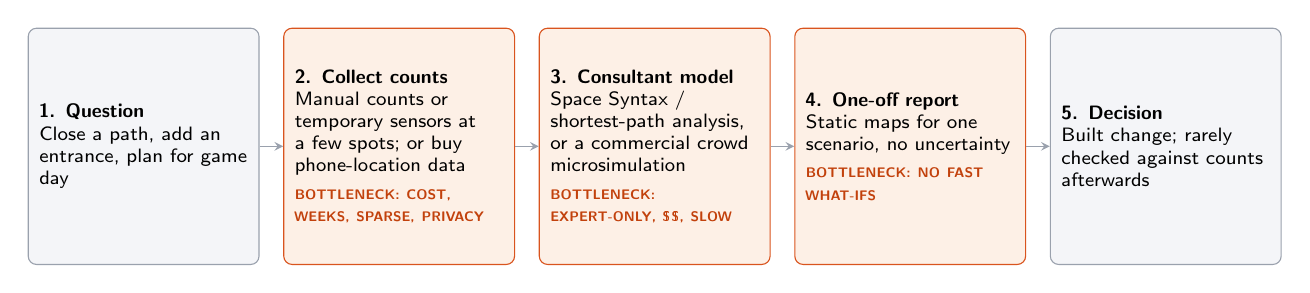
\begin{tikzpicture}[node distance=0.4cm]
  \node[stage=2.65cm, tall] (q) at (0,0) {\textbf{1. Question}\\ Close a path, add an entrance, plan for game day};
  \node[stage=2.65cm, tall, bn, right=0.3cm of q.north east, anchor=north west] (c) {\textbf{2. Collect counts}\\ Manual counts or temporary sensors at a few spots; or buy phone-location data\bnlabel{BOTTLENECK: COST, WEEKS, SPARSE, PRIVACY}};
  \node[stage=2.65cm, tall, bn, right=0.3cm of c.north east, anchor=north west] (m) {\textbf{3. Consultant model}\\ Space Syntax / shortest-path analysis, or a commercial crowd microsimulation\bnlabel{BOTTLENECK: EXPERT-ONLY, \$\$, SLOW}};
  \node[stage=2.65cm, tall, bn, right=0.3cm of m.north east, anchor=north west] (r) {\textbf{4. One-off report}\\ Static maps for one scenario, no uncertainty\bnlabel{BOTTLENECK: NO FAST WHAT-IFS}};
  \node[stage=2.65cm, tall, right=0.3cm of r.north east, anchor=north west] (d) {\textbf{5. Decision}\\ Built change; rarely checked against counts afterwards};
  \foreach \a/\b in {q/c,c/m,m/r,r/d} \draw[flow] (\a.east) -- (\b.west);
\end{tikzpicture}
\caption{Current planner workflow. Orange steps are bottlenecks. Typical turnaround: weeks to months per scenario.}
\end{figure}

\textbf{Bottlenecks in the current process:} data collection (cost, lead time, few locations, privacy for phone data); expert-only modelling; one scenario per study; no uncertainty; no check of outcomes after the change is built.

\begin{figure}[H]
\centering
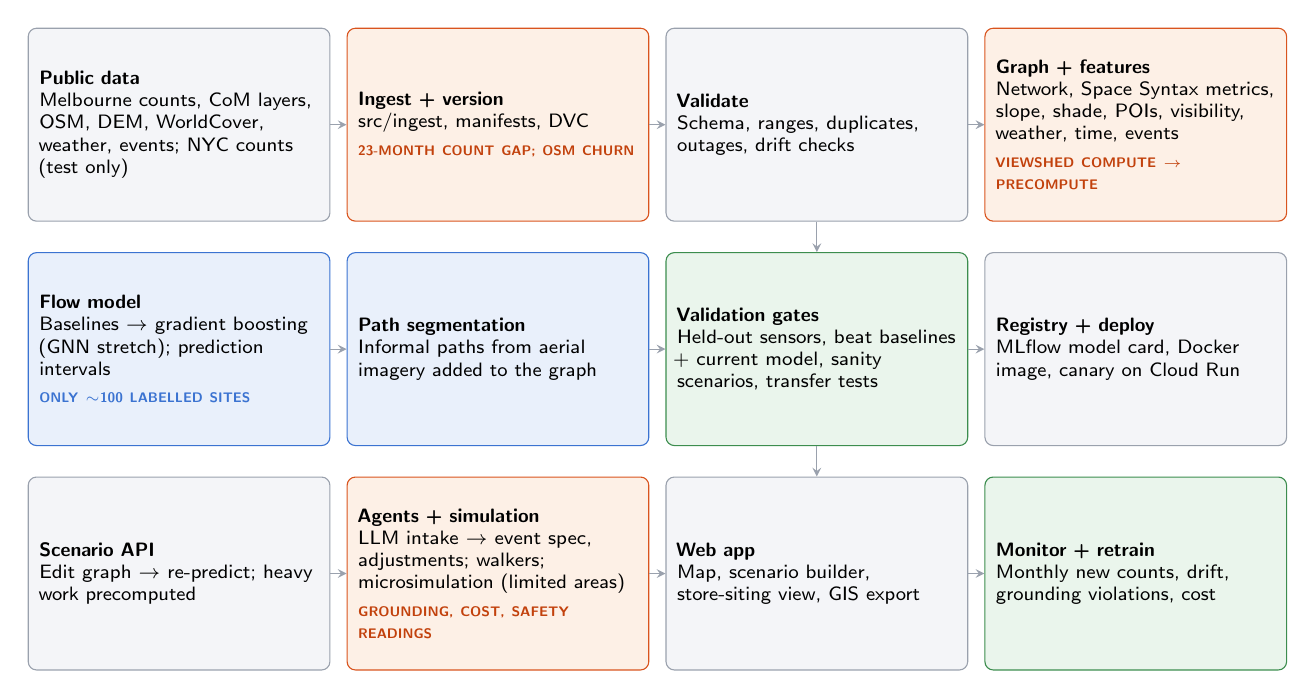
\begin{tikzpicture}
  \def\w{3.55cm}\def\gx{4.05}\def\gy{2.85}
  % Row 1
  \node[stage=\w] (a1) at (0,0) {\textbf{Public data}\\ Melbourne counts, CoM layers, OSM, DEM, WorldCover, weather, events; NYC counts (test only)};
  \node[stage=\w, bn] (a2) at (\gx,0) {\textbf{Ingest + version}\\ src/ingest, manifests, DVC\bnlabel{23-MONTH COUNT GAP; OSM CHURN}};
  \node[stage=\w] (a3) at (2*\gx,0) {\textbf{Validate}\\ Schema, ranges, duplicates, outages, drift checks};
  \node[stage=\w, bn] (a4) at (3*\gx,0) {\textbf{Graph + features}\\ Network, Space Syntax metrics, slope, shade, POIs, visibility, weather, time, events\bnlabel{VIEWSHED COMPUTE $\rightarrow$ PRECOMPUTE}};
  % Row 2
  \node[stage=\w, ml] (b1) at (0,-\gy) {\textbf{Flow model}\\ Baselines $\rightarrow$ gradient boosting (GNN stretch); prediction intervals\mllabel{ONLY $\sim$100 LABELLED SITES}};
  \node[stage=\w, ml] (b2) at (\gx,-\gy) {\textbf{Path segmentation}\\ Informal paths from aerial imagery added to the graph};
  \node[stage=\w, gate] (b3) at (2*\gx,-\gy) {\textbf{Validation gates}\\ Held-out sensors, beat baselines + current model, sanity scenarios, transfer tests};
  \node[stage=\w] (b4) at (3*\gx,-\gy) {\textbf{Registry + deploy}\\ MLflow model card, Docker image, canary on Cloud Run};
  % Row 3
  \node[stage=\w] (c1) at (0,-2*\gy) {\textbf{Scenario API}\\ Edit graph $\rightarrow$ re-predict; heavy work precomputed};
  \node[stage=\w, bn] (c2) at (\gx,-2*\gy) {\textbf{Agents + simulation}\\ LLM intake $\rightarrow$ event spec, adjustments; walkers; microsimulation (limited areas)\bnlabel{GROUNDING, COST, SAFETY READINGS}};
  \node[stage=\w] (c3) at (2*\gx,-2*\gy) {\textbf{Web app}\\ Map, scenario builder, store-siting view, GIS export};
  \node[stage=\w, gate] (c4) at (3*\gx,-2*\gy) {\textbf{Monitor + retrain}\\ Monthly new counts, drift, grounding violations, cost};
  \foreach \r in {a,b,c}{
    \draw[flow] (\r1.east) -- (\r2.west); \draw[flow] (\r2.east) -- (\r3.west); \draw[flow] (\r3.east) -- (\r4.west);}
  \draw[flow] (a3.south) -- (b3.north);
  \draw[flow] (b3.south) -- (c3.north);
\end{tikzpicture}

\vspace{2pt}
{\scriptsize\color{gray}
\tikz\draw[bnline,fill=bnfill] (0,0) rectangle (0.25,0.18); Bottleneck / risk \quad
\tikz\draw[mlline,fill=mlfill] (0,0) rectangle (0.25,0.18); ML models \quad
\tikz\draw[gateline,fill=gatefill] (0,0) rectangle (0.25,0.18); Quality gates / feedback loop \quad
Turnaround target: seconds per scenario}
\caption{Proposed Stoa pipeline. Rows read left to right, top to bottom.}
\end{figure}

\textbf{Bottlenecks in our pipeline and how we address them:}

\begin{xltabular}{\linewidth}{|L{3.6cm}|Y|Y|}
\hline\hrow
\textbf{Bottleneck} & \textbf{Why} & \textbf{Improvement} \\\hline
\endhead
Few labelled sites ($\sim$100 sensors) & Limits what a model can learn about unsensed paths & Network features share information along the graph; spatial CV; calibration curve; strong baselines as a floor \\\hline
Transfer to new sites & Only one city of dense ground truth; volumes, ice, campus rhythms and seasons differ elsewhere & Transferable features; shape vs.\ scale with per-site calibration; within-Melbourne and NYC transfer tests (Section~\ref{sec:transfer}) \\\hline
23-month count gap & Two separate eras of data & Use as a temporal robustness test; era feature \\\hline
Viewshed and network-metric compute & Ray-casting and centrality are expensive per scenario & Precompute baseline values; recompute only the affected neighbourhood on edits \\\hline
LLM cost, latency and grounding & Per-interaction calls are slow and costly; risk of invented numbers & Call the LLM only for intake and final narration; grounding checker blocks untraceable numbers \\\hline
Source churn (OSM edits, API changes) & Segment IDs and schemas drift & Stable ID mapping; schema validation; last-good snapshot fallback \\\hline
Model latency on large networks & Re-predicting thousands of segments per edit can exceed target latency & Sub-graph slicing, aggressive caching, and batch prediction optimization \\\hline
Microsimulation compute and ground truth & Physics-style crowds are expensive, and Melbourne counts validate flows, not crowd dynamics & Limited areas only; existing open-source simulator; controlled-experiment data for validation, reported separately \\\hline
Live demo failure & Live model and LLM calls can fail in front of an audience & Cached replay mode: record real runs and replay them during the expo \\\hline
\end{xltabular}

% =====================================================================
\section{Metrics, Objectives, and Business Goals}

\subsection{Key Metrics}

\begin{xltabular}{\linewidth}{|L{3.0cm}|Y|L{4.2cm}|}
\hline\hrow
\textbf{Component} & \textbf{Metric} & \textbf{Reported on} \\\hline
\endhead
Flow model & MAE and RMSE on log1p(count); median absolute \% error; Spearman rank correlation across segments per hour & Held-out sensors (spatial CV + final test) \\\hline
Flow model & \% improvement over shortest-path betweenness and Space Syntax + calibration & Same held-out sensors \\\hline
Flow model & Prediction interval coverage (nominal 80\%) and width & Held-out sensors \\\hline
Flow model & Event-day error and peak hour bias, reported separately & AFL match days (Marvel Stadium; MCG coverage weak) \\\hline
Flow model & Calibration curve: error vs number of local sensors & Simulated new-site setting in Melbourne; NYC \\\hline
Transfer (within city) & Spearman rank correlation and MAE on log counts, uncalibrated and calibrated on 1--2 sensors & Held-out Melbourne precincts (UniMelb edge, Carlton, North Melbourne) \\\hline
Transfer (cross city) & Spearman rank correlation across locations per period; error on log period totals before and after calibrating on $k$ locations & NYC DOT bi-annual counts \\\hline
Flow model (equity) & Error by urban-density tier & Held-out sensors grouped by density \\\hline
Scenarios & Sanity-scenario pass rate & Scenario test suite \\\hline
Microsimulation & Speed--density relation and flow through bottlenecks vs measured values, reported separately from the flow model & Controlled pedestrian-experiment data \\\hline
Knowledge adjustments & Change in post-opening error when the Metro Tunnel opening is entered as a planner statement & Melbourne sensors near the new stations \\\hline
Workflow & Technical decisions and time to first scenario, vs a Space Syntax workflow & Scripted comparison; optional small usability test \\\hline
Path segmentation & IoU / F1; recall of known paths & Held-out tiles \\\hline
Intake agent & Field-level extraction accuracy; location placement accuracy; grounding violation rate & tests/agent\_eval/ \\\hline
System & p95 API latency; error rate; cost per scenario; pipeline success rate & Production monitoring \\\hline
\end{xltabular}

\subsection{Objectives}
\begin{enumerate}
  \item Predict hourly pedestrian volume on every segment of a site, with calibrated uncertainty, more accurately than the standard Space Syntax baseline.
  \item Answer a planning what-if in seconds instead of weeks.
  \item Run as a reproducible MLOps system: versioned data, tracked experiments, gated releases, monitoring and automatic retraining.
  \item Measure how the approach transfers: to unfamiliar areas within Melbourne, to a new city (NYC), and with a few local counts for calibration. Demonstrate it on a site without sensors (NEU campus) and on event days.
  \item Simulate crowds: route-sampling walkers everywhere, and microsimulation in limited outdoor areas, validated separately against controlled-experiment data.
  \item Answer store-siting questions: hourly and weekly pass-by at candidate storefronts.
\end{enumerate}

\subsection{Alignment with Business Goals}
\begin{itemize}
  \item \textbf{Lower cost per decision:} fewer manual counts and consultant studies per scenario.
  \item \textbf{Better decisions:} more options tested, with uncertainty shown, before money is spent on construction.
  \item \textbf{Comfort and access:} slope, shade and climate features show where routes are hard for older people or people with disabilities, or uncomfortable in heat.
  \item \textbf{Event operations:} approach-street planning for game days, with crowd simulation at egress zones and station approaches.
  \item \textbf{Store siting:} independent owners ask how many people pass a candidate storefront, and when. Existing tools (Placer.ai, FootfallCam's location analysis app, GrowthFactor) mostly rely on phone data or installed counters and are priced for chains; Stoa is privacy-safe, works without sensors and is affordable for independent owners. The UI states that pass-by is not walk-in, that exposure is visible impressions rather than customers, and that a store changes the traffic around it.
  \item \textbf{Signage (stretch):} street-level signs and billboards for pedestrians, using the same exposure score plus sign size, height, viewing angle, occlusion and readability. Outdoor-advertising audiences are already measured for vehicles (e.g.\ Geopath in the US); our angle is pedestrian, 3D, and before installation.
  \item \textbf{Market \& Business Model:} city and campus planners and event organisers; per-site calibration is the path to new customers via a B2B SaaS model offering tiered subscriptions based on site area and API usage. The calibration curve tells a customer how many counters they need.
\end{itemize}

% =====================================================================
\section{Failure Analysis}

\subsection{Project Risks (during development)}

\begin{xltabular}{\linewidth}{|L{4.4cm}|L{2.0cm}|Y|}
\hline\hrow
\textbf{Risk} & \textbf{Likelihood} & \textbf{Mitigation} \\\hline
\endhead
Learned model does not beat the Space Syntax baseline & Medium & Gradient-boosted model fully evaluated by week 4; checkpoint in week 6; feature ablations; report honestly. The GNN is a stretch goal adopted only if it beats the gradient-boosted model \\\hline
Counts licence field empty on the portal & Low & Portal-wide terms put all CoM open data under CC BY 4.0; credit the City of Melbourne \\\hline
Overfitting to sensor locations & Medium & Spatially blocked CV; untouched final test sensors; no location identifiers as features \\\hline
Model ranks well but misses volumes in a new city & High & Report rank and scale separately; per-site calibration; show the calibration curve rather than claim zero-shot accuracy \\\hline
Effects absent from Melbourne (ice, class-change surges) & Certain & Labelled hand-set rule or omission; state the gap in the UI and report \\\hline
Portable model much weaker than the Melbourne-rich one & Medium & Report the gap honestly; calibration on local counts; keep Melbourne-only layers for Melbourne accuracy \\\hline
Metro Tunnel opening (2025-11-30) shifts recent counts near the new stations & Certain & Station entrances with opening dates in the graph; split results at the opening or add a station-access feature \\\hline
Losing count history (the portal keeps only $\sim$2 years) & Certain without action & Merge-only ingest; dated snapshot; DVC versions of every pull \\\hline
Scope creep (3D, agents, segmentation, microsimulation) & High & Scope guardrails; GNN, 3D walk views and the planning assistant moved to stretch; microsimulation in two stages on an existing simulator; integrate the viewshed as precomputed features first \\\hline
Microsimulation read as a safety assessment & Medium & Outdoor approach areas only, never venue interiors; planning-guidance wording enforced in the UI and agent text \\\hline
No crowd-dynamics ground truth in Melbourne & Certain & Validate microsimulation on controlled-experiment data and report it separately from the flow model \\\hline
No ground truth at NEU & Certain & Present NEU as a demonstration only; accuracy claims rest on Melbourne; transfer claims rest on the Melbourne and NYC tests \\\hline
Cloud budget overrun & Medium & Cloud Run scale-to-zero; budget alerts; precompute; no per-click LLM calls \\\hline
\end{xltabular}

\subsection{Pipeline Failures and Mitigations}

\begin{xltabular}{\linewidth}{|L{2.6cm}|Y|Y|}
\hline\hrow
\textbf{Stage} & \textbf{Failure mode} & \textbf{Detection $\rightarrow$ mitigation} \\\hline
\endhead
Ingest & API down, schema change, partial download & HTTP/schema checks, .part files, checksums $\rightarrow$ last-good snapshot, alert \\\hline
Validation & Sensor outage, relocation, duplicates, impossible values & Range/freshness/level-shift checks $\rightarrow$ quarantine sensor, stop on hard failures \\\hline
Graph build & OSM edit breaks segment IDs or connectivity & Stable ID mapping, connectivity tests $\rightarrow$ keep previous graph \\\hline
Training & Run fails or regresses & MLflow tracking; gates vs baselines and current model $\rightarrow$ do not register \\\hline
Deployment & New model worse in production & Canary traffic split, live error checks $\rightarrow$ automatic rollback \\\hline
Serving & Latency spikes, cold starts & p95 alerts $\rightarrow$ min instances for the API, cached precomputed results \\\hline
Agents & Invented numbers, wrong place, prompt injection & Grounding checker blocks output; map confirmation; structured outputs only \\\hline
\end{xltabular}

\subsection{Risks After Deployment}
\begin{itemize}
  \item \textbf{Drift:} new developments, construction closures, or behaviour change after events like COVID. Detect through monthly accuracy on new counts and input drift; retrain.
  \item \textbf{Misuse:} forecasts or crowd simulations read as safety guarantees, or pass-by read as expected customers. Mitigate with UI and agent wording rules, visible uncertainty bands, and labelled assumptions for user adjustments.
  \item \textbf{Transfer error:} a new site behaves differently from Melbourne, most of all in absolute volume. Mitigate with per-site calibration, the measured transfer results and calibration curve to set expectations, and a visible flag when a site's features fall outside the training range.
\end{itemize}

% =====================================================================
\section{Deployment Infrastructure}

\begin{figure}[H]
\centering
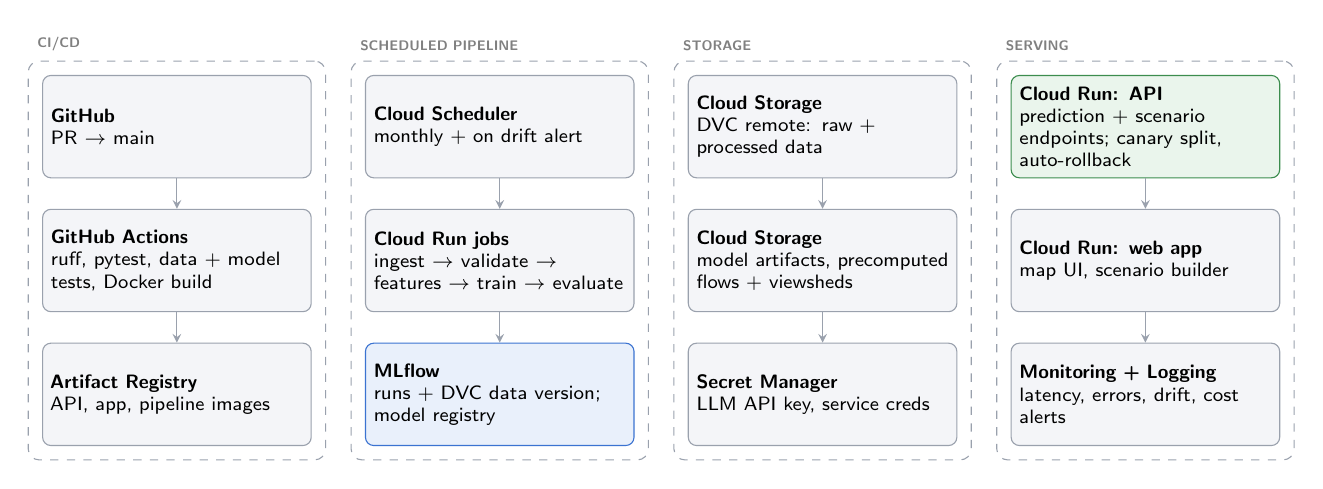
\begin{tikzpicture}[
  dep/.style={draw=boxline, fill=boxgray, rounded corners=3pt, align=left, text width=3.2cm,
              inner sep=3pt, font=\scriptsize, minimum height=1.3cm,
              execute at begin node={\hyphenpenalty=10000\exhyphenpenalty=10000}},
  col/.style={draw=boxline, dashed, rounded corners=4pt, inner sep=5pt},
  coltitle/.style={font=\tiny\bfseries\color{gray}, anchor=south west}]
  \def\gx{4.1}\def\gy{1.7}
  % CI/CD
  \node[dep] (g1) at (0,0) {\textbf{GitHub}\\ PR $\rightarrow$ main};
  \node[dep] (g2) at (0,-\gy) {\textbf{GitHub Actions}\\ ruff, pytest, data + model tests, Docker build};
  \node[dep] (g3) at (0,-2*\gy) {\textbf{Artifact Registry}\\ API, app, pipeline images};
  % Pipeline
  \node[dep] (p1) at (\gx,0) {\textbf{Cloud Scheduler}\\ monthly + on drift alert};
  \node[dep] (p2) at (\gx,-\gy) {\textbf{Cloud Run jobs}\\ ingest $\rightarrow$ validate $\rightarrow$ features $\rightarrow$ train $\rightarrow$ evaluate};
  \node[dep, draw=mlline, fill=mlfill] (p3) at (\gx,-2*\gy) {\textbf{MLflow}\\ runs + DVC data version; model registry};
  % Storage
  \node[dep] (s1) at (2*\gx,0) {\textbf{Cloud Storage}\\ DVC remote: raw + processed data};
  \node[dep] (s2) at (2*\gx,-\gy) {\textbf{Cloud Storage}\\ model artifacts, precomputed flows + viewsheds};
  \node[dep] (s3) at (2*\gx,-2*\gy) {\textbf{Secret Manager}\\ LLM API key, service creds};
  % Serving
  \node[dep, draw=gateline, fill=gatefill] (v1) at (3*\gx,0) {\textbf{Cloud Run: API}\\ prediction + scenario endpoints; canary split, auto-rollback};
  \node[dep] (v2) at (3*\gx,-\gy) {\textbf{Cloud Run: web app}\\ map UI, scenario builder};
  \node[dep] (v3) at (3*\gx,-2*\gy) {\textbf{Monitoring + Logging}\\ latency, errors, drift, cost alerts};
  \foreach \c in {g,p,s,v}{\draw[flow] (\c1) -- (\c2); \draw[flow] (\c2) -- (\c3);}
  \begin{scope}[on background layer]
    \foreach \c in {g,p,s,v}{
      \node[col, fit=(\c1)(\c3)(\c1.west |- v1.north)(\c3.west |- v3.south)] (c\c) {};}
  \end{scope}
  \node[coltitle] at (cg.north west) {CI/CD};
  \node[coltitle] at (cp.north west) {SCHEDULED PIPELINE};
  \node[coltitle] at (cs.north west) {STORAGE};
  \node[coltitle] at (cv.north west) {SERVING};
\end{tikzpicture}

\vspace{2pt}
{\scriptsize\color{gray} Flow: a merge to main builds images $\rightarrow$ the gated model from the MLflow registry ships to the API as a canary $\rightarrow$ monitoring drives retraining through Cloud Scheduler. Orchestration is not final yet: Cloud Scheduler + Cloud Run jobs (shown) or Airflow on a small VM.}
\caption{Deployment on Google Cloud.}
\end{figure}

\begin{xltabular}{\linewidth}{|L{3.8cm}|Y|}
\hline\hrow
\textbf{Component} & \textbf{Role} \\\hline
\endhead
GitHub + GitHub Actions & Lint (ruff), tests (pytest incl.\ data and model tests), Docker builds, deploy on merge to main \\\hline
Artifact Registry & Container images for the API, web app and pipeline jobs \\\hline
Cloud Scheduler + Cloud Run jobs & Proposed orchestration: Cloud Scheduler triggering Cloud Run jobs (alternative: Airflow on a small VM; Cloud Composer is too costly): monthly ingest $\rightarrow$ validate $\rightarrow$ features $\rightarrow$ train $\rightarrow$ evaluate, plus drift-triggered runs \\\hline
Cloud Storage & DVC remote (data), model artifacts, precomputed baseline flows and viewsheds \\\hline
MLflow & Experiment tracking (with DVC data version) and model registry with model cards \\\hline
Cloud Run (API) & Prediction and scenario endpoints; one Docker image bundles the model, the feature pipeline (same code as training) and the viewshed engine; canary rollout with automatic rollback; per-site calibrated variants stored separately \\\hline
Cloud Run (web app) & Map, scenario builder, store-siting view, results; cached replay mode for the expo (3D walk views are a stretch goal) \\\hline
Secret Manager & LLM API key and service credentials; nothing hard-coded \\\hline
Cloud Monitoring + Logging & Latency, errors, drift metrics, cost and budget alerts \\\hline
\end{xltabular}

\textbf{Supported platforms:} web app on current desktop Chrome, Edge, Firefox and Safari (tablet for viewing); REST API (JSON) for integration; GIS exports (GeoJSON, GeoPackage, CSV) for QGIS/ArcGIS in research mode. Development on macOS and Linux with Python 3.11+ and Docker.

% =====================================================================
\section{Monitoring Plan}

\begin{xltabular}{\linewidth}{|L{3.6cm}|Y|Y|}
\hline\hrow
\textbf{What we monitor} & \textbf{Why} & \textbf{How / trigger} \\\hline
\endhead
Accuracy on each month's new Melbourne counts & The only live ground truth & Per-sensor error vs the training-time error; retrain when error rises beyond a set margin \\\hline
Input drift & Weather, calendar and feature distributions shift & PSI / KS tests per feature; alert on sustained drift \\\hline
Prediction drift & Network-wide volumes shift unexpectedly & Distribution of predictions per hour band vs reference \\\hline
Out-of-range sites & A deployed site's features (volumes, climate, network) fall outside Melbourne's training range & Per-site feature range check at deploy and on each scenario; flag predictions as lower confidence \\\hline
Network changes & New OSM path edits or closures invalidate the graph & Diff each OSM snapshot; rebuild the graph and re-run sanity scenarios \\\hline
Data freshness and quality & Silent outages corrupt training & Last-update age per source; sensor outage counts \\\hline
Agent quality & Wrong parses erode trust & User correction rate on parsed fields; grounding violations (target 0); location confirmations \\\hline
Service health and cost & Usability and budget & p95 latency, error rate, cost per scenario, LLM token spend, budget alerts \\\hline
\end{xltabular}

Retraining runs monthly on new counts, when accuracy drops or drift is detected, and per site when a customer adds new counts. Every retrained model re-runs all validation gates, including the transfer tests, before canary deployment.

% =====================================================================
\section{Success and Acceptance Criteria}

\begin{enumerate}
  \item Flow model beats both baselines on held-out sensors: $\geq$~15\% lower MAE on log counts than Space Syntax + calibration.
  \item Prediction intervals are calibrated: 80\% intervals cover 75--85\% of held-out observations.
  \item Event-day error is reported separately, and no event-day claim is made without it.
  \item Transfer is reported, not assumed: within-Melbourne precinct results are reported uncalibrated and calibrated on 1--2 sensors, NYC results uncalibrated and along the calibration curve, and no claim beyond Melbourne is made without them. Goal (not a pass/fail criterion): on NYC, rank correlation across locations $\geq$~0.6 uncalibrated, and error on log totals halved after calibrating on 5 locations.
  \item 100\% of sanity scenarios pass before any deployment.
  \item Microsimulation validation is reported separately from the flow model, against controlled-experiment data.
  \item Path segmentation: recall $\geq$~0.7 on known informal paths in held-out tiles.
  \item Intake agent: $\geq$~90\% field-level accuracy on tests/agent\_eval/, and zero grounding violations reach the user.
  \item System: p95 latency $\leq$~2\,s for precomputed scenarios; the full pipeline runs end to end from the scheduler with no manual steps; a bad canary is rolled back automatically in a staged test.
  \item Reproducibility: any reported number can be regenerated from a git commit + DVC version + MLflow run.
  \item Demonstrations: NEU campus, one event scenario with crowd simulation, and the store-siting view run end to end in the web app (or from cached replay), with their known gaps (ice, class-change surges) stated on screen.
\end{enumerate}

% =====================================================================
\section{Timeline Planning}

\textit{Preliminary; dates align with course deliverables and milestones.}

\begin{xltabular}{\linewidth}{|L{1.3cm}|L{3.0cm}|Y|}
\hline\hrow
\textbf{Week} & \textbf{Dates (2026)} & \textbf{Deliverables} \\\hline
\endhead
1 & Sep 28 -- Oct 4 & Scoping; data audit; ingest scripts for all sources (done) \\\hline
2 & Oct 5 -- 11 & DVC + GCS remote (first: version the rolling counts table); unified counts table; validation checks; freeze graph, feature-table, event-spec and adjustment interfaces \\\hline
3 & Oct 12 -- 18 & Graph build from the CoM network and an OSM-derived Melbourne graph; features v1; baselines (betweenness, Space Syntax + calibration); spatial CV harness with transfer-precinct folds \\\hline
4 & Oct 19 -- 25 & Gradient-boosted flow model fully evaluated: held-out sensors, baselines, intervals, transfer precincts; MLflow tracking; NYC graph around the count locations \\\hline
5 & Oct 26 -- Nov 1 & Calibration curve (Melbourne and NYC); portable model and NYC cross-city test; event-day evaluation; route-sampling walkers v1 \\\hline
6 & Nov 2 -- 8 & Checkpoint: model vs baselines decision. Integration dry run (data $\rightarrow$ features $\rightarrow$ model $\rightarrow$ API $\rightarrow$ map). Segmentation dataset; intake agent eval set; API skeleton \\\hline
7 & Nov 9 -- 15 & Segmentation model; intake agent (event specs and knowledge adjustments); microsimulation set-up on an open-source simulator for one limited area \\\hline
8 & Nov 16 -- 22 & Scenario API with sanity scenarios; viewshed features; web app v1 with the store-siting view and exposure score; Docker image; CI/CD; Cloud Run deploy \\\hline
9 & Nov 23 -- 29 & Microsimulation validation against controlled-experiment data; Metro Tunnel knowledge-adjustment test; monitoring, drift detection, retraining trigger \\\hline
10 & Nov 30 -- Dec 6 & NEU campus, event and store-siting demos; cached replay mode; canary/rollback test; documentation \\\hline
11 & Dec 7 -- 11 & Final report, model cards, presentation \\\hline
\end{xltabular}

% =====================================================================
\section{Additional Information}

\subsection{Scope Guardrails}

\textbf{In scope:} flow model (gradient-boosted), transfer tests (within-Melbourne precincts and NYC), crowd simulation (route-sampling walkers, then microsimulation in limited outdoor areas), path segmentation (campus scale), LLM intake agent with knowledge adjustments, event days, viewshed integration, store-siting view, MLOps loop, web app.

\textbf{Stretch goals (Tier 2):} spatio-temporal GNN, LLM planning assistant, 3D walk views, Melbourne and Boston marathon case studies, research mode with a terrain-grid graph builder, pedestrian signage placement, a new-store before/after study (case-study scale), Fenway validation, cross-campus transfer demonstration (NEU Oakland).

\textbf{Out of scope (future work):} inverse reinforcement learning, venue interiors, city-wide microsimulation, class-change surge modelling, learned ice and snow effects.

\subsection{Open Decisions}
\begin{itemize}
  \item Open-source microsimulator (e.g.\ JuPedSim or Vadere), after checking licences
  \item Graph and feature-table formats
  \item Orchestration tool (Cloud Scheduler + Cloud Run jobs vs Airflow on a VM)
  \item Weather source (proposed: ERA5 via Open-Meteo)
  \item Ice in Boston predictions: labelled hand-set rule, or omit
\end{itemize}

\textbf{To verify:} simulator licences; availability of controlled pedestrian-experiment data (e.g.\ the J\"ulich archive); Melbourne Marathon route against sensor locations and which race years fall in the data; MBTA gated-entry data for the Boston Marathon demonstration.

\subsection{Data Findings from the Initial Audit}
\begin{itemize}
  \item A hand-exported counts file contained only $\sim$9\% of the real records. The full data is pulled directly from the API and archive.
  \item The portal's standard GeoJSON export of the pedestrian network drops every attribute. The full-attribute ZIP is used instead.
  \item Open 1\,m terrain is not available for Melbourne (state LiDAR is licensed or non-commercial). The GA 5\,m DEM plus surveyed CoM footpath slopes cover the need.
  \item 30\,m global elevation models read 20--27\,m too high in the CBD (they measure rooftops), so they are not used for slope.
  \item Three Melbourne sensors on Swanston St at the University of Melbourne's edge (IDs 42--44, running since 2015) follow the academic calendar: $\sim$0.45$\times$ their weekday mean in January and December, $\sim$1.6$\times$ in March. CBD sensors barely change across the year. This justifies an academic-term feature and a campus-like transfer test inside Melbourne.
  \item NYC DOT's bi-annual counts (114 locations, 2007--May 2026) are period totals from two days a year, not hourly series; the transfer test compares them with summed predictions over the same hours. NYC's continuous automated counts cover only four pedestrian sites.
  \item The live Melbourne counts table is a rolling $\sim$2-year window: by 2026-10-04 the portal had already dropped a day we hold. Ingest now merges instead of overwriting.
  \item Usable history is thinner than ``2009--2022'' suggests: 24\% of archive rows are in the 2020--21 COVID period, only 43 sensors have five or more non-COVID years, and North Melbourne's archive sensors start in 2020--22.
  \item No sensor lies within 500\,m of the MCG; event-day evaluation rests on Marvel Stadium.
  \item The Metro Tunnel (opened 2025-11-30) shows in the data: sensors within 300\,m of the new stations rose a median $\sim$4.5\% year on year while others were flat. The 2019 CoM network has no station entrances.
  \item Every outdoor sensor is within 18\,m of a walkable CoM link (median 2\,m), so sensor-to-edge matching is feasible, but each sensor has $\sim$3 candidate links within 10\,m and needs a hand check.
  \item A before/after test of new stores is feasible only as case studies: of 133 large openings in the business census, 7 have a sensor within 100\,m with counts before and after, and none is clean. The one strong case is Emporium Melbourne (2014), with sensors 164--191\,m away.
  \item Opening hours are sparse: $\sim$12\% of OSM amenities and shops in the study area carry them, and the CoM datasets have none, so ``open now'' is a partial feature with explicit missingness.
\end{itemize}

\subsection{Tech Stack}

Python 3.11+, pandas, GeoPandas, rasterio, LightGBM, PyTorch (segmentation, viewshed; PyTorch Geometric for the stretch GNN), an open-source pedestrian simulator, DVC, MLflow, FastAPI, Docker, GitHub Actions, Google Cloud (Cloud Run, Cloud Storage, Artifact Registry, Secret Manager, Cloud Scheduler), a web map front end (MapLibre / deck.gl), and an LLM API for the agents. Documentation in Markdown and LaTeX.

\end{document}
